\begin{tikzpicture}[
    every node/.style={node distance=2mm, inner sep=0, outer sep=0},
    image/.style={}
]
    \node[image] (img1) {
        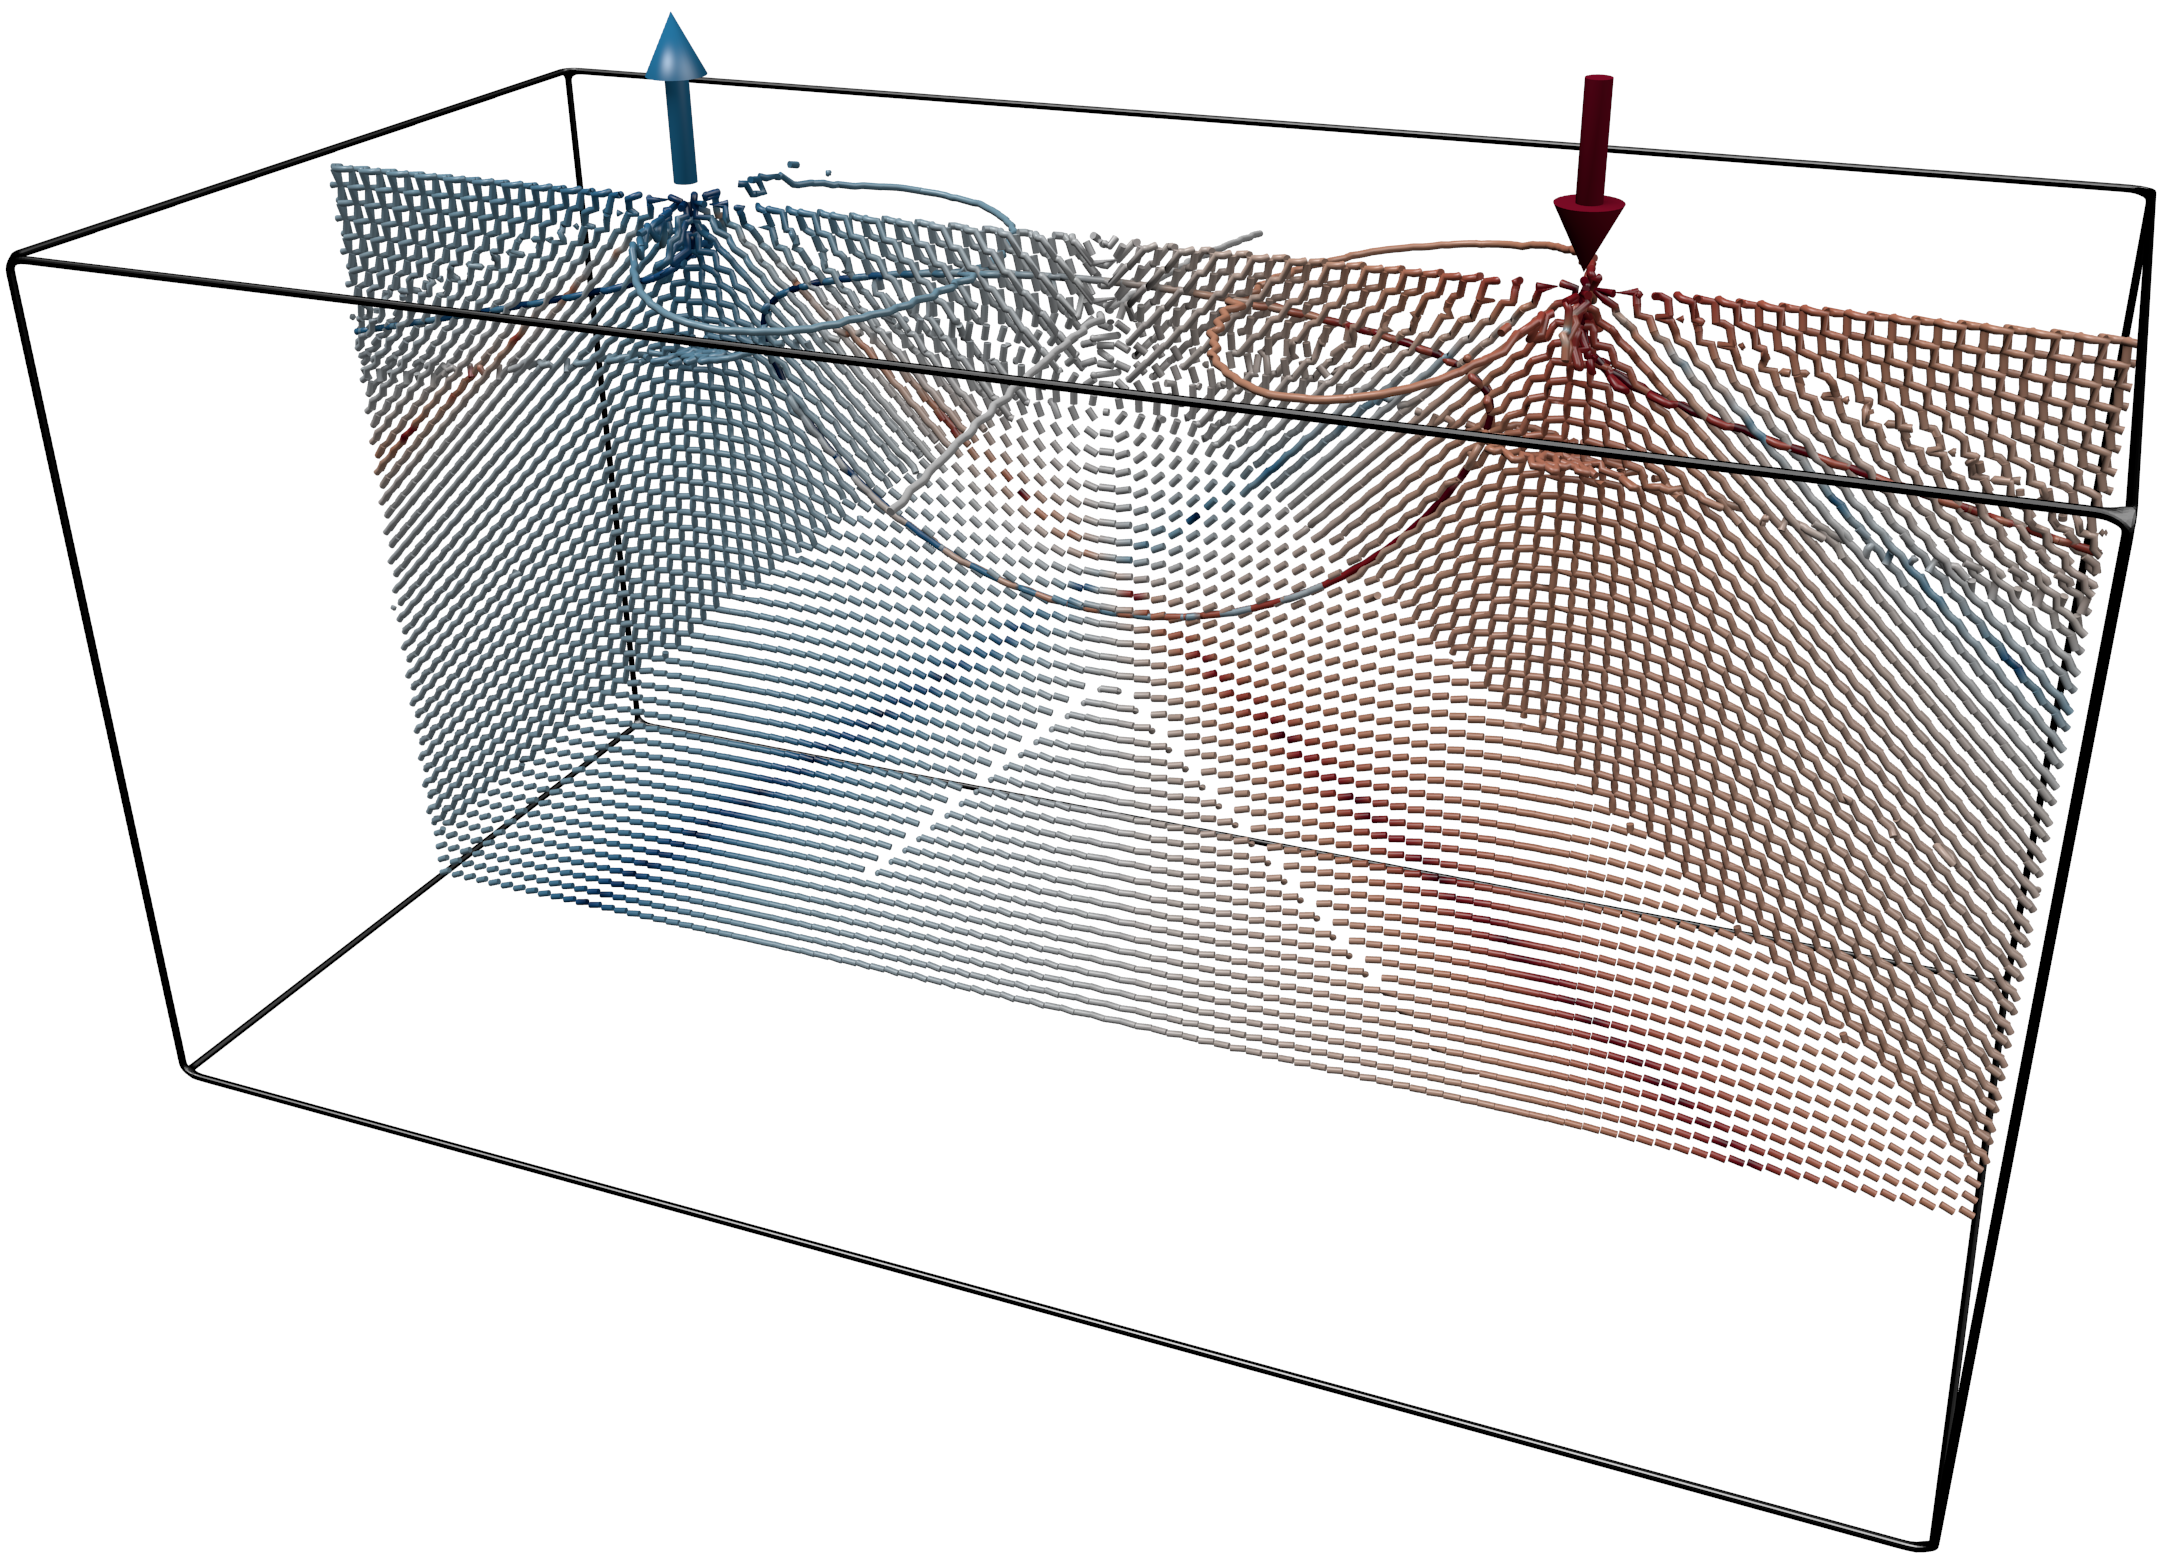
\includegraphics[width=\figurewidth]{figures/PointLoad_total}
    };
    % \begin{scope}[
    %     shift=(img1.south west), % origin is lower left corner
    %     x={($(img1.south east)-(img1.south west)$)}, % x axis is lower side
    %     y={($(img1.north west)-(img1.south west)$)}] % y axis is left side
    %     % \draw[help lines, opacity=0.5, xstep=.01,ystep=.01] (0,0) grid (1,1);
    %     % \draw[thin, xstep=.1,ystep=.1] (0,0) grid (1,1);
    %     % \foreach \x in {0,...,9} { \node [anchor=north] at (\x/10,0) {0.\x}; }
    %     % \foreach \y in {0,...,9} { \node [anchor=east] at (0,\y/10) {0.\y}; }
    %     \draw[mycolor4, thick, rotate around={10:(0.24, 0.81)}]
    %         (0.24, 0.81) ellipse (0.09 and 0.02);
    %     \draw[mycolor4, thick] (0.45, 0.825) circle[radius=5pt];
    %     \draw[mycolor4, thick] (0.51, 0.795) circle[radius=5pt];
    % \end{scope}
    % \node[image, below=of img1.south west, anchor=north west] (img2) {
    %     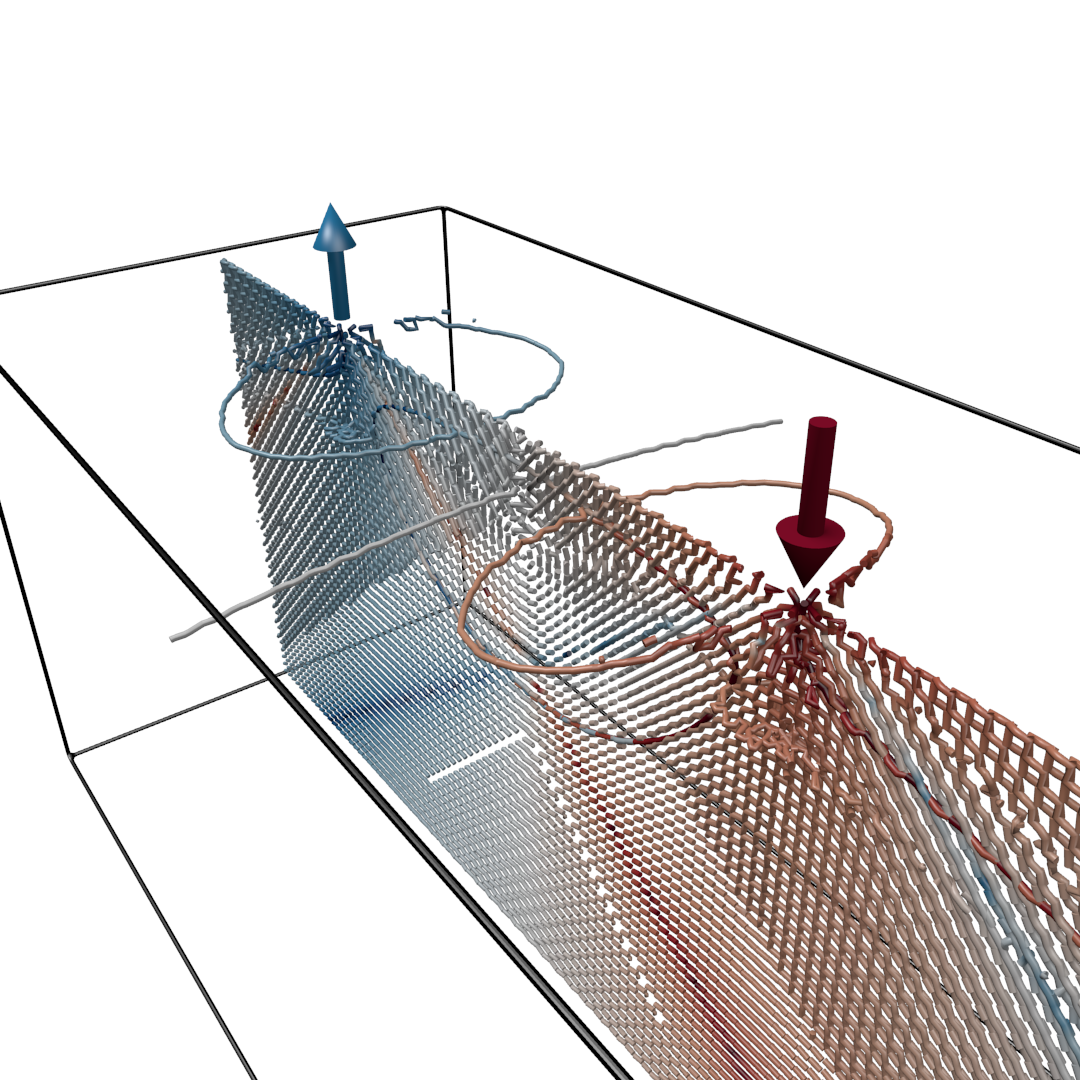
\includegraphics[width=0.5\figurewidth-2mm/2]{figures/PointLoad_detail1_sq}
    % };
    % \begin{scope}[
    %     shift=(img2.south west), % origin is lower left corner
    %     x={($(img2.south east)-(img2.south west)$)}, % x axis is lower side
    %     y={($(img2.north west)-(img2.south west)$)}] % y axis is left side
    %     % \draw[help lines, opacity=0.5, xstep=.01,ystep=.01] (0,0) grid (1,1);
    %     % \draw[thin, xstep=.1,ystep=.1] (0,0) grid (1,1);
    %     % \foreach \x in {0,...,9} { \node [anchor=north] at (\x/10,0) {0.\x}; }
    %     % \foreach \y in {0,...,9} { \node [anchor=east] at (0,\y/10) {0.\y}; }
    %     % \draw[red, thick, rotate around={-45:(0.85, 0.27)}]
    %     %     (0.85, 0.27) ellipse (0.2 and 0.05);
    %     % \draw[red, thick, rotate around={15:(0.62, 0.47)}]
    %     %     (0.62, 0.47) ellipse (0.23 and 0.1);
    %     % \draw[red, thick, rotate around={7:(0.36, 0.64)}]
    %     %     (0.36, 0.64) ellipse (0.19 and 0.08);
    %     % \draw[red, thick, rotate around={20:(0.44, 0.51)}]
    %     %     (0.44, 0.51) ellipse (0.32 and 0.04);
    %     % \draw[red, thick] (0.45, 0.6) circle[radius=5pt];
    %     % \draw[red, thick] (0.5, 0.54) circle[radius=5pt];
    %     % \draw[red, thick] (0.55, 0.53) circle[radius=5pt];
    % \end{scope}
    \node[image, anchor=south west] (img3)
        at (img1.south west) {
        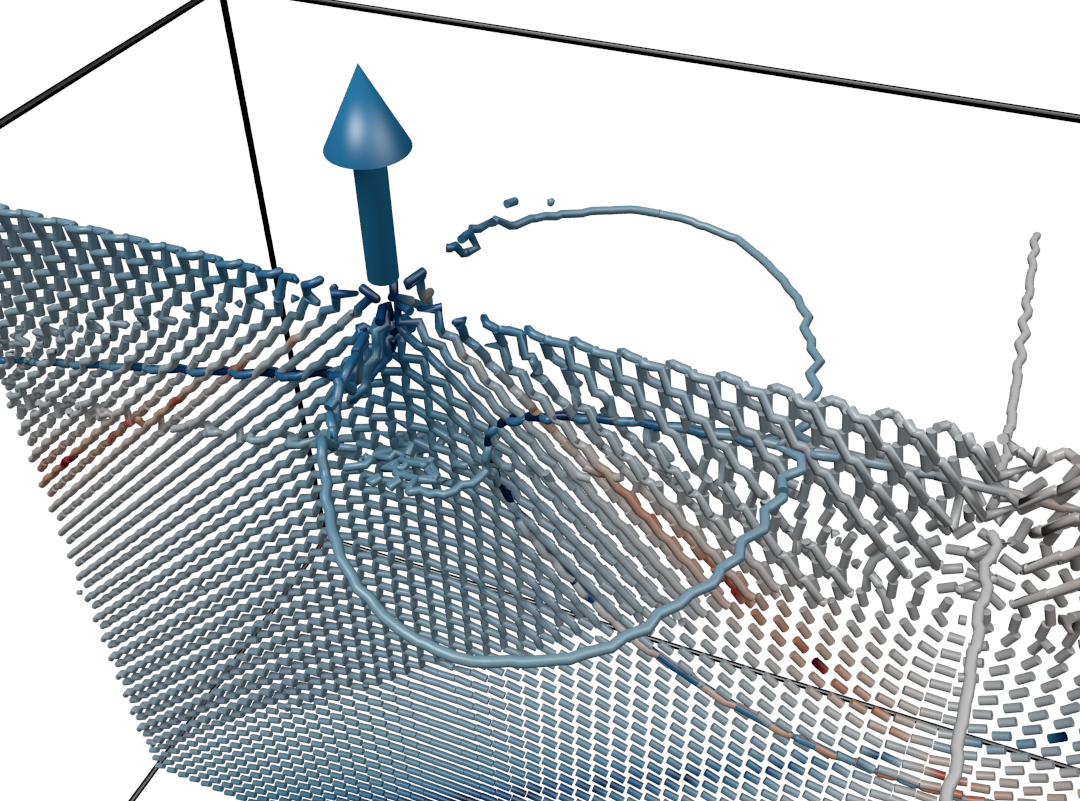
\includegraphics[width=0.5\figurewidth]{figures/PointLoad_detail2}
    };
    \draw[draw=white, line width=3pt]
        (img3.north west) -- (img3.north east) -- (img3.south east);
    \begin{scope}[
        shift=(img3.south west), % origin is lower left corner
        x={($(img3.south east)-(img3.south west)$)}, % x axis is lower side
        y={($(img3.north west)-(img3.south west)$)}] % y axis is left side
        % \draw[help lines, opacity=0.5, xstep=.01,ystep=.01] (0,0) grid (1,1);
        % \draw[thin, xstep=.1,ystep=.1] (0,0) grid (1,1);
        % \foreach \x in {0,...,9} { \node [anchor=north] at (\x/10,0) {0.\x}; }
        % \foreach \y in {0,...,9} { \node [anchor=east] at (0,\y/10) {0.\y}; }
        \draw[mycolor4, thick, rotate around={-2:(0.16, 0.54)}]
            (0.16, 0.54) ellipse (0.15 and 0.02);
        \draw[mycolor4, thick] (0.74, 0.43) circle[radius=5pt];
        \draw[mycolor4, thick] (0.91, 0.35) circle[radius=5pt];
    \end{scope}
\end{tikzpicture}